\documentclass[10pt,a4paper]{article}
\usepackage[margin=22mm]{geometry}
\usepackage[T1]{fontenc}
\usepackage{lmodern,amsmath,amssymb,booktabs,graphicx,tikz,hyperref,fvextra}
\usetikzlibrary{arrows.meta,positioning,calc,decorations.pathmorphing}
\definecolor{ink}{RGB}{20,53,78}
\hypersetup{colorlinks=true,urlcolor=ink,linkcolor=ink}
\setlength{\parindent}{0pt}
\setlength{\parskip}{5pt}
\emergencystretch=3em

\title{\color{ink}A feedback loop with a communication delay}
\author{}
\date{Original learning collection -- November 2026}
\begin{document}
\begin{center}{\LARGE\color{ink}A feedback loop with a communication delay}\\[5pt]{\small Original learning collection -- November 2026}\end{center}

\textbf{Evidence note.} Original teaching scenario. Numerical parameters are deliberately chosen for learning. All generated data and curves are synthetic; no physical measurement is asserted.
\section{Design brief}
The normalized tracking loop is $L(s)=8/[s(s+3)]$. Find gain crossover $\omega_c$, phase margin $\phi_m$ and the first constant pure-delay stability boundary. Introduce delays $T=0.10\,\mathrm{s}$ and $0.30\,\mathrm{s}$. Compare fifth-order Pade approximation with exact phase $-\omega T$, explaining the scope of the rational approximation.
\section{Physical system}
\begin{center}\resizebox{\ifdim\width>.98\linewidth.98\linewidth\else\width\fi}{!}{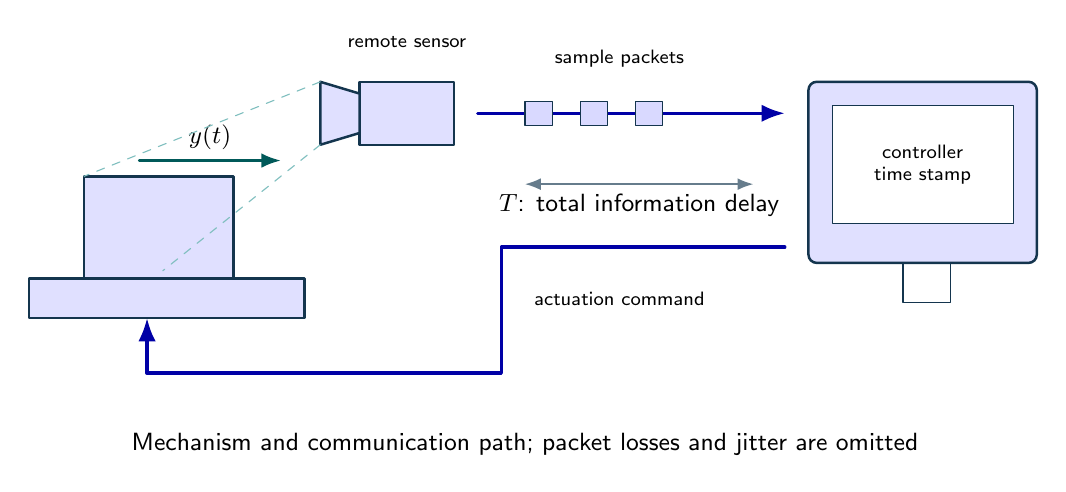
\begin{tikzpicture}[
font=\sffamily\small,>=Latex,line cap=round,line join=round,
wall/.style={draw=ink,line width=1.2pt,fill=blue!5},
water/.style={fill=cyan!25,draw=none},
metal/.style={draw=ink,fill=blue!12,line width=.9pt},
flow/.style={->,draw=blue!65!black,line width=1.2pt},
heat/.style={->,draw=orange!85!black,line width=1.1pt},
measure/.style={->,draw=teal!70!black,line width=.9pt},
dim/.style={<->,draw=ink!65,line width=.6pt},
spring/.style={draw=ink,decorate,decoration={coil,aspect=.5,segment length=4pt,amplitude=3pt}},
wire/.style={draw=ink,line width=1pt},
lab/.style={align=center,font=\sffamily\small},
smalllab/.style={align=center,font=\sffamily\scriptsize}]

\draw[metal](.5,1)rectangle(4,1.5);
\draw[metal](1.2,1.5)rectangle(3.1,2.8);
\draw[measure](1.9,3)--(3.7,3)node[midway,above]{$y(t)$};
\draw[metal](4.7,3.2)rectangle(5.9,4);
\draw[metal](4.7,3.35)--(4.2,3.2)--(4.2,4)--(4.7,3.85)--cycle;
\draw[teal!50,dashed](4.2,3.2)--(2.2,1.6)(4.2,4)--(1.2,2.8);
\node[smalllab]at(5.3,4.5){remote sensor};
\draw[metal,rounded corners=3pt](10.4,1.7)rectangle(13.3,4);
\draw[fill=white,draw=ink](10.7,2.2)rectangle(13,3.7);
\draw[ink](11.6,1.7)--(11.6,1.2)--(12.2,1.2)--(12.2,1.7);
\node[smalllab]at(11.85,2.95){controller\\time stamp};
\draw[flow](6.2,3.6)--(10.1,3.6);
\foreach \x in {6.8,7.5,8.2}{\draw[fill=blue!15,draw=ink](\x,3.45)rectangle++(.35,.3);}
\node[smalllab]at(8,4.3){sample packets};
\draw[flow](10.1,1.9)--(6.5,1.9)--(6.5,.3)--(2,.3)--(2,1);
\node[smalllab]at(8,1.25){actuation command};
\draw[dim](6.8,2.7)--node[below]{$T$: total information delay}(9.7,2.7);
\node[lab]at(6.8,-.6){Mechanism and communication path; packet losses and jitter are omitted};
\end{tikzpicture}
}\par{\small A remote mechanism sends measurements and receives commands through a communication path. The model combines those latencies into one ideal constant delay; the drawn packet train is not an experimental record.}\end{center}
\section{Gain crossover}
The open-loop magnitude is $8/[\omega\sqrt{\omega^2+9}]$. Setting it to one and defining $z=\omega^2$ gives $z^2+9z-64=0$, hence
\[\omega_c=\sqrt{\frac{-9+\sqrt{337}}2}.\]
The phase is $-90^\circ-\tan^{-1}(\omega/3)$, so the no-delay phase margin is $90^\circ-\tan^{-1}(\omega_c/3)$.
\section{Delay consumes phase}
A pure delay multiplies the loop by $e^{-sT}$. Its frequency magnitude is one and its phase is $-\omega T$ radians. Therefore crossover does not move and
\[PM(T)=PM(0)-\omega_cT\frac{180}{\pi},\qquad T_{crit}=\frac{PM(0)\pi/180}{\omega_c}.\]
This is the first imaginary-axis crossing for this stable nominal closed loop with its single positive gain crossover. It is not a universal rule for arbitrary loops with multiple crossings.
\section{Rational approximation}
The fifth-order Pade model approximates the delay by a rational all-pass transfer function. Compare its phase at crossover with the exact phase before using its time response. Artificial right-half-plane zeros and high-order dynamics are approximation features, not physical actuator modes.
\section{Design decision}
Reserve phase for unmodeled sensor and actuator dynamics rather than spending the entire mathematical delay budget. Packet loss, variable delay and sampled-data effects are outside a constant-delay continuous-time approximation.
\section{What to learn from the experiment}
Exact delay phase supplies the stability-budget calculation. Pade models are checked approximations used to visualize nominal responses.
\section{System sketch}
\begin{center}\resizebox{\ifdim\width>.98\linewidth.98\linewidth\else\width\fi}{!}{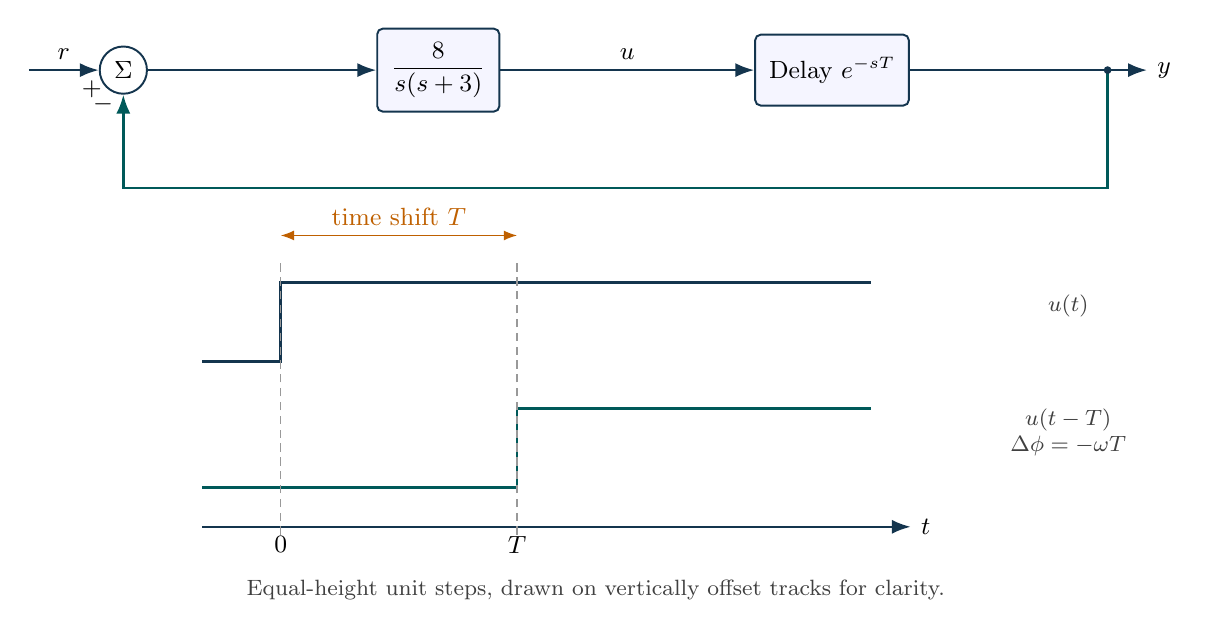
\begin{tikzpicture}[x=1cm,y=1cm,>=Latex,font=\small,
block/.style={draw=ink,fill=blue!4,rounded corners=2pt,minimum height=9mm,align=center,line width=.7pt,inner sep=5pt},
sum/.style={circle,draw=ink,fill=white,minimum size=6mm,inner sep=0pt,line width=.7pt},
sig/.style={->,draw=ink,line width=.85pt},
fb/.style={->,draw=teal!70!black,line width=.85pt},
dist/.style={->,draw=orange!75!black,line width=.85pt},
tap/.style={circle,fill=ink,inner sep=1.4pt},
note/.style={font=\footnotesize,align=center,text=black!75}]

\node[sum](e)at(1,2.1){$\Sigma$};
\node[block](g)at(5,2.1){$\dfrac{8}{s(s+3)}$};
\node[block](d)at(10,2.1){Delay $e^{-sT}$};
\draw[sig](-.2,2.1)--node[above]{$r$}node[pos=.9,below]{$+$}(e);
\draw[sig](e)--(g);\draw[sig](g)--node[above]{$u$}(d);
\draw[sig](d)--(14,2.1)node[right]{$y$};
\draw[fb](13.5,2.1)--(13.5,.6)--(1,.6)--node[pos=.9,left]{$-$}(e);
\fill[ink](13.5,2.1)circle(1.4pt);
\draw[sig](2,-3.7)--(11,-3.7)node[right]{$t$};
\draw[line width=1pt,draw=ink](2,-1.6)--(3,-1.6)--(3,-.6)--(10.5,-.6);
\draw[line width=1pt,draw=teal!70!black](2,-3.2)--(6,-3.2)--(6,-2.2)--(10.5,-2.2);
\draw[densely dashed,black!40](3,-3.8)--(3,-.35)(6,-3.8)--(6,-.35);
\node[below]at(3,-3.7){$0$};\node[below]at(6,-3.7){$T$};
\draw[<->,orange!75!black](3,0)--node[above]{time shift $T$}(6,0);
\node[note]at(13,-.9){$u(t)$};
\node[note]at(13,-2.5){$u(t-T)$\\$\Delta\phi=-\omega T$};
\node[note]at(7,-4.5){Equal-height unit steps, drawn on vertically offset tracks for clarity.};

\end{tikzpicture}
}
\par\small\refstepcounter{figure}\label{fig:system}\textbf{Figure \thefigure.} Constant pure delay shifts a signal in time and contributes frequency-dependent phase lag. The sketch shows ideal steps, not experimental records.\end{center}
\section{Executed computational evidence}
\VerbatimInput[fontsize=\small,breaklines=true]{results.txt}
\begin{center}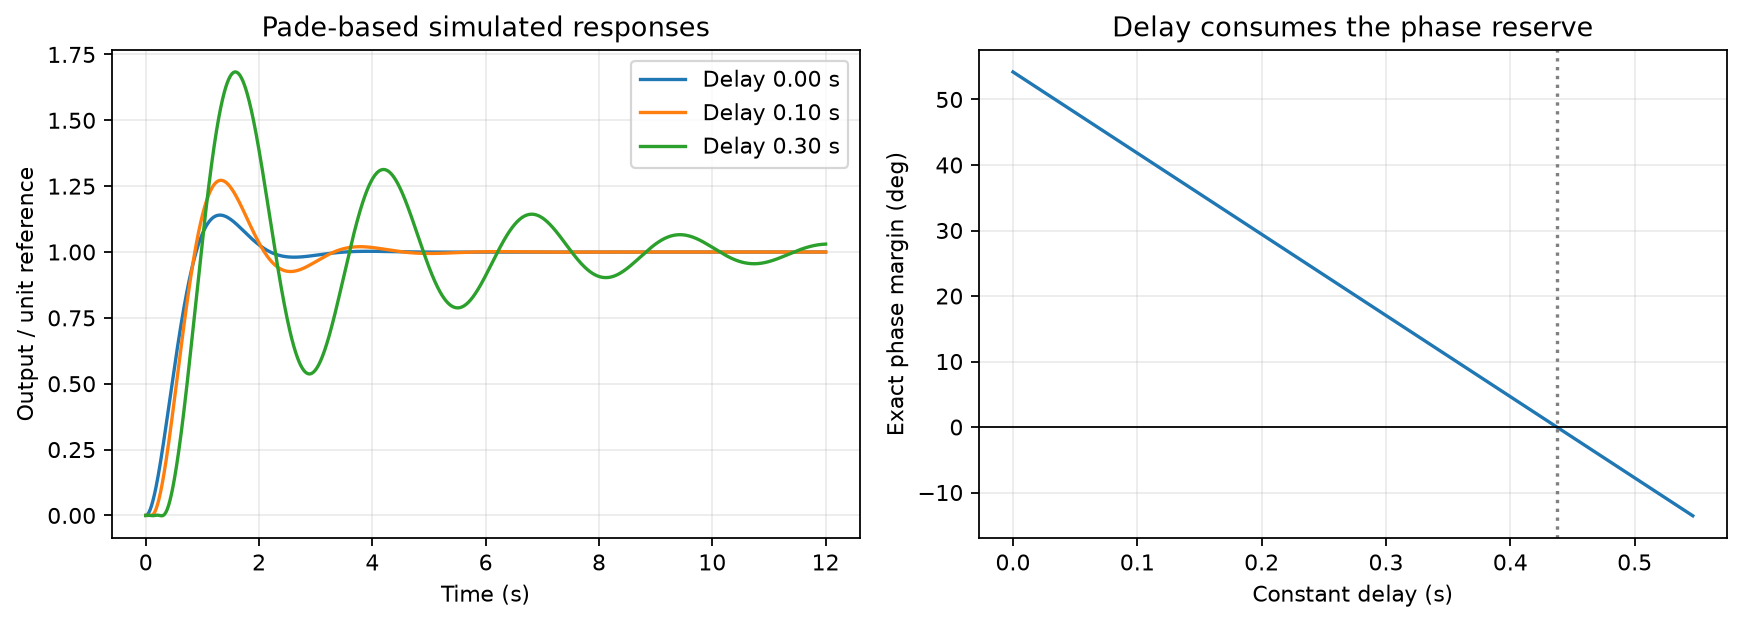
\includegraphics[width=\linewidth,height=.46\textheight,keepaspectratio]{response.png}\end{center}
\section{Method references}
The equations use standard balance laws and feedback-control methods. Further explanation: \url{https://apmonitor.com/pdc/} and \url{https://fbsbook.org/}. Implementation documentation: \url{https://python-control.readthedocs.io/en/0.10.2/}. See the repository reference catalog for individual topics and videos.
\end{document}
